\section{FRAMEWORK UMBRELLA ARCHITECTURE AND DESIGN}
%This is a summary of section 2 in the Hoffman paper

\begin{figure*}[t]
\centering
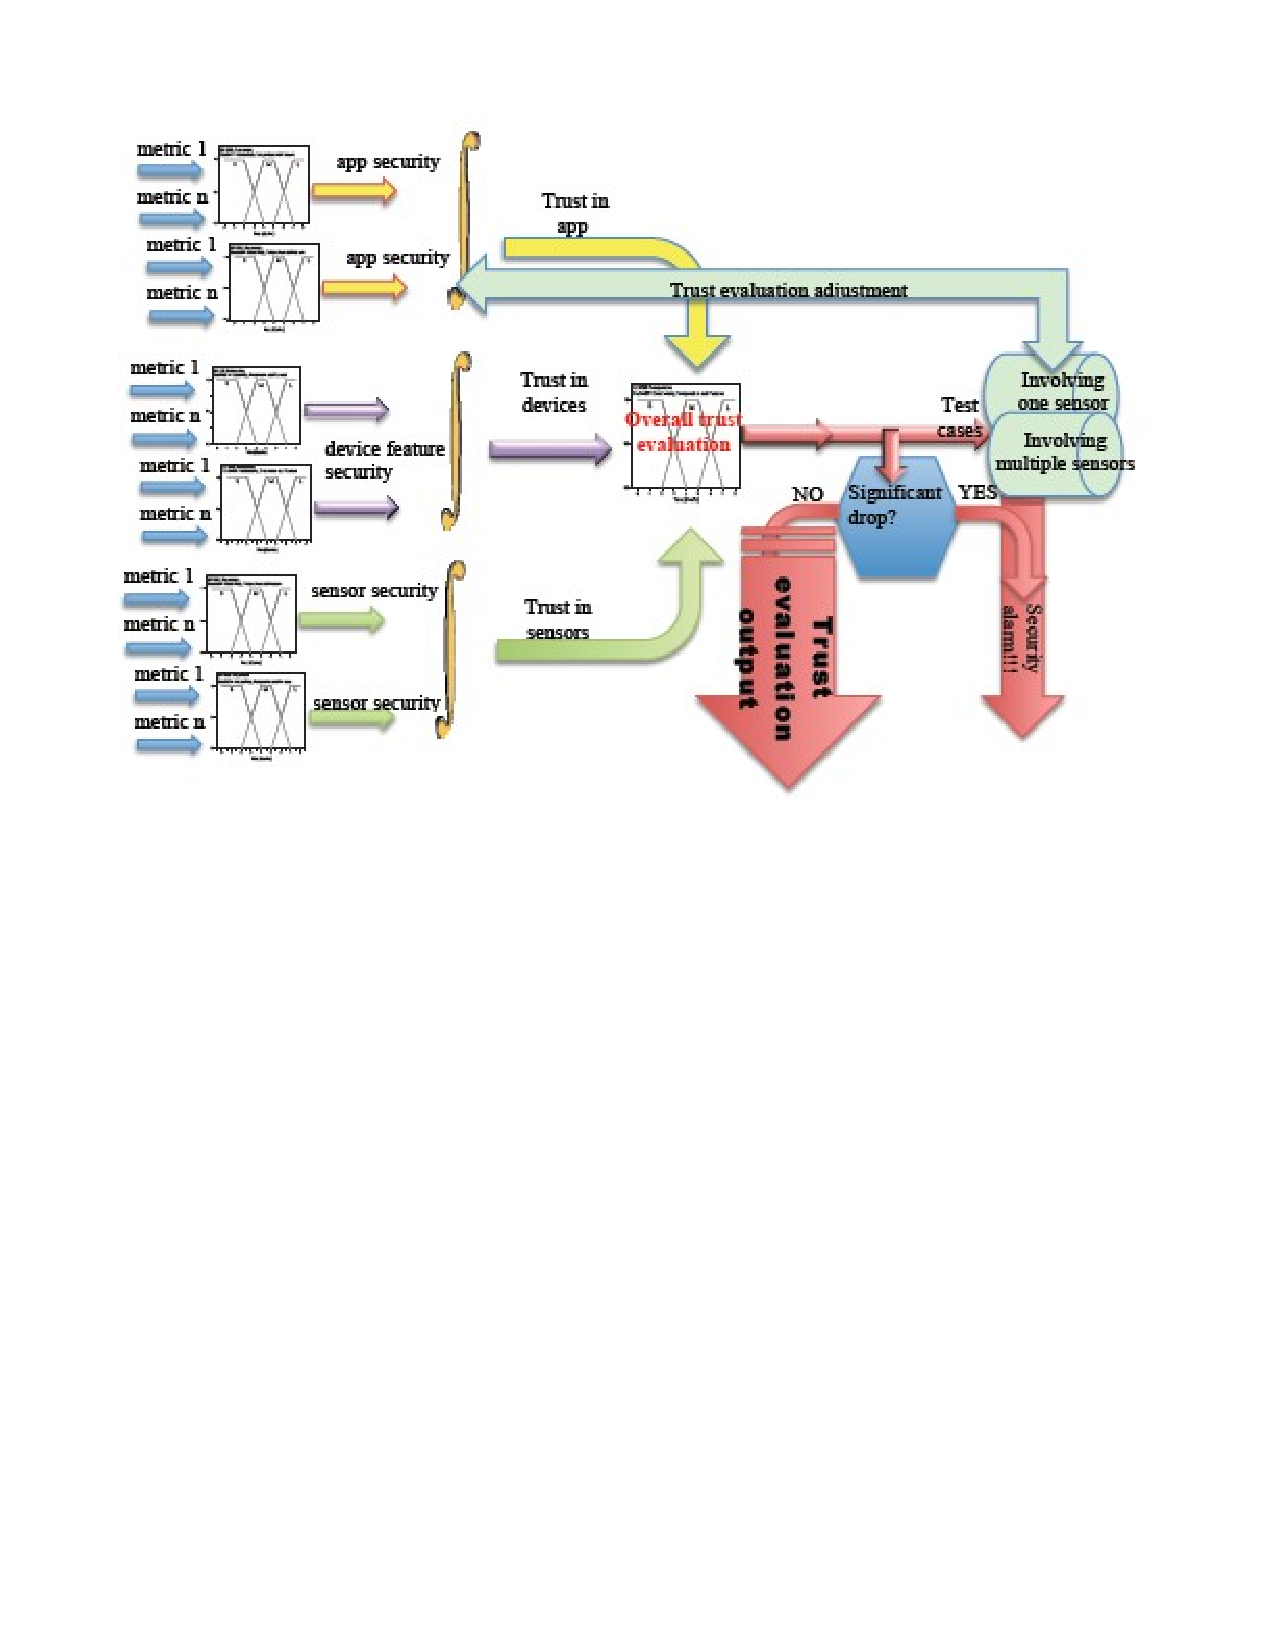
\includegraphics[width=7.0in]{umbrella_framework.pdf}
\caption{Framework operation and architecture.}
\label{fig:umbrella}
\end{figure*}

A hierarchical trust analysis can look at the entire system and combine measurements from multiple sources, making
it more powerful than measuring a single component or layer.
This section discusses a comprehensive mechanism that provides a scalable and extendable methodology of trust
 evaluation and analysis which is implemented on Android-based mobile devices. \weiss{why is it limited to Android?}
Trust evaluation of a mobile smartphone device is a complex subject, which depends on multiple characteristics, 
e.g. sensor accuracy, the rate of encrypted messages, \weiss{I don't understand that one}
 and/or the probability of a system's breakdown over a given period of time. Its evaluation should integrate various metrics ranging from the accuracy and reliability of the data sources to the security of the procedures and tools used. The major research challenge of the framework design is integrating the numerous metrics needed to characterize a device's trustworthiness while working with limited resources and processing power. 
We address this challenge by hierarchically structuring the composition of trust metrics as well as by designing a specialized calculus to evaluate the overall trust metric. 
Therefore, the major innovative emphasis in our framework design is put on the integration of a wide variety of indicators and their evaluation procedures. The framework procedures output the overall trust evaluation indicators and additionally calculate the individual product of metrics characterizing system features which are then used to produce recommendations for improvement. The trust evaluation will facilitate decision-making, improve performance and increase accountability through the collection, analysis, and reporting of relevant performance-related data. This design facilitates the framework extension through
 the inclusion of other metrics, as well as the ease of modification and improvement (see fig~\ref{fig:umbrella})
Current implementation of this framework provides the following metric functionality: 

\begin{enumerate}
\item Analysis of the installed applications through the application-specific metadata provided by the Play store. Applications represent the largest security and privacy risk to a device and user's data. The data provided by the Play store leverages the experiences of millions of users and holds all data associated with the distribution of an application including its associated documentation. The Play store also provides meta-information about applications which gives useful characteristic data about an application. These data can be used to assess an individual application's risk. Rules were generated to classify each application into a risk impact class based on this meta-data. The combined trust classes of all applications installed on a device would be used to create a security risk rating for the whole device.

\item The usage verification of security tools embedded into the operating system and proper preventative security practices. Android provides users with many different tools which increase the security and privacy of their devices in addition to updates 
to patch exposed vulnerabilities.  When properly used, these tools improve the security of the devices. They are 
intended to gather a 
comprehensive overview of the software running on a mobile device by analyzing the operating system and user settings. 
First the operating system is checked to confirm that it is running the most recent version available. Second the personal 
security settings on the device are examined to determine if the user is utilizing the appropriate tools to secure the device. 
These operating system verification checks combined generate a score, which is used in the security and privacy framework operation result.

\item The trust evaluation based on the level of privacy provided.  
The spurious output of a device's internal sensors can sometimes indicate the existence of a privacy/security problem 
%Verifying the validity of the sensors can detect security and quality problems of the device 
that would be missed by the other metrics. Most mobile devices now come equipped with a variety of sophisticated 
internal and external sensors which are capable of very accurate measurements of their surrounding environment. 
As the data from these sensors are used in more security critical applications the importance that these data remain accurate and legitimate should not be underestimated. For example, data from the GPS sensor can be verified to be trustworthy and assigned a trust rating. The combination of ratings from all sensors would produce the devices sensor trust score.
% privacy: disclosing the user's exact location.  Users have only very coarse-grained control
% an app that uses Google map service would most likely request this in the manifest file.
\end{enumerate}


Unlike other reported tools available, our framework has an umbrella structure that allows for integration of 
diverse trust evaluation mechanisms and results through a rule-based classification system.
This open architecture can also be extended to include 
 self-learning capabilities to allow for its optimization towards a particular device and a criteria set. Each of these procedures given above generates a security risk rating, which is then integrated into the umbrella framework. This framework takes into account the varied landscape of mobile devices and is designed to be flexible and easily adaptable to the changing security environment. Based on this design and contribution of each of the procedures could be adjusted depending on the target.

\subsection{Rule-based Classification}
The goal is to assign a trust level to an application based on usage patterns (this is a part of the
overall trust evaluation hierarchy).
The classifications are: 
\begin{enumerate}
  \item Low trust: These applications are considered to have
a low trust evaluation and a high probability of its negative
impact on the overall device security
  \item Moderate trust: These applications are evaluated to have
less negative  impact on the overall device security
  \item High trust: These applications are considered to have a high
trust evaluation or a low probability of  negative impact
on the overall device security.
\end{enumerate}

We evaluate overall trust based on a separate
analysis of each application. On the first step the list of all
applications installed on the device is compiled. After that the
manifest file for each application installed is analyzed in order to
fetch the application name, package name, required features,
version, required permission, path info, date on which the
application was installed and the target SDK version. This
information is used to evaluate  trust according to the classification.
However, this is refined using
application category. This information could
be retrieved from the Google Play store. The Google Play store
holds all data associated with the distribution of an application
including its APK file and associated documentation.  Following
features can be retrieved from the
meta-data:
\begin{itemize}
  \item Number of Installs – Total number of installs across the apps life
  \item Number of Reviews – Total number of reviews from unique users
  \item Score – User rating of 1.0 to 5.0
  \item Developer – Name of the developer
  \item Permissions – Which resources can be accessed by the app
\end{itemize}

The first three fields can be used to find an application’s
popularity which when matched with a history of values shows
user trend information.  Although it may not be possible to determine if an
application is a security risk based on this
information, data from a large number of users could be very reliable~\cite{}.

it can be used in rules in combination with other data~\cite{jing2014riskmon}.

Here are some examples of rules that are used in the classification: 
\begin{itemize}
  \item If number of downloads were low with low ratings, the
    application was classified as low trust.
  \item If the number of downloads were low with good application
    score, the application was classified as moderate trust.
  \item If the application had low recent score it was classified as moderate trust
    stating that there was something wrong with the latest patch released by the developer.
  \item If the application was from a unknown publisher with low score
    and low number of downloads it was classified as low trust.
  \item If the application was from an unknown publisher with high
    number of downloads and high score it was classified as moderate trust.
\end{itemize}
